\documentclass[main]{subfiles}
\begin{document}

%@@@@@@@@@@@@@@@@@@@@@@@@@@@@@@
%\noindent
%\textbf{Topics: Hopfield Networks - 28.11.2019} \\
%Lecturer: Dr. Matthew Cook \\
%Author: Vanessa Leite \{vanessa at ini.uzh.ch\}

\section{Hopfield Networks}

The Hopfield Networks, or Hopfield Model, was proposed by John Hopfield in the early 80s.
He thought about connecting units to each other in an all-to-all pattern.
When we look into the brain and how neurons are connected to each other, we do not see always a clear pathway, i.e., is hard to think about the connections in the brain in terms of input-output.

\paragraph{Characteristics of Hopfield Networks}
\begin{itemize}[noitemsep,nolistsep]
	\item Every node is connected to every other node but not to itself.
	\item Connection weights are symmetric.
	\item $\sum x_i w_i < 0$ represents an inactive unit, $\sum x_i w_i \geq 0$ is active.
	\item Entire Network is in some state at any time. Set of active units of the entire network is important.
	\item Some states are stable and some are not. While in an unstable state, updating the network leads to a state change.
	\item Stable state is a local minimum. This does however not have to happen.
	\item Bias is an unit that is always on.
	\item Weight symmetry of a connection is correlated to the frequency of neurons firing together (following Hebbian learning).
\end{itemize}

\subsection{Hopfield and Memory}

We are used to think about computation as a process that receives an input, does something and generate an output.
However, this is not we see in our memories, for instance.
It seems our memory works with Pattern Completion, also known as Content Addressable Memory or Associative Memory.
This memory has no input-output relation: given any piece of it, we can recover the rest.
Hopfield Networks can be used to give us insights about how the memory works by having a highly connected network that computes with no input-output, but with states.

\begin{itemize}[noitemsep,nolistsep]
	\item A Hopfield Network is an associative type of memory. Information is stored in the stable states as local minima.
	\item It is important that information is distinct.
	\item Associative memory has room for error but is still recognizable. Convergence to nearby stable states.
	\item If some units are retrievable and all others are set randomly, the correct units will eventually set the wrong units right.
\end{itemize}

\begin{figure}[H]
	\centering
	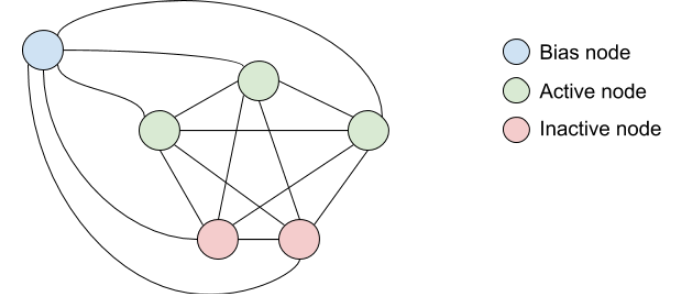
\includegraphics[width=0.5\textwidth]{hopfield-network-basic.png}
	\caption{Model of a Hopfield Network. Red units are inactive, green units are active, blue unit is the bias node that is always active.}
\end{figure}

\subsection{Updates and State Dynamics}

Maximize the sum of active weights (weights between active units) is the dynamic of Hopfield Network (updating the output of one unit at time). This results in a stable state. We update everything but the bias node (bias node are always active and do not change their state).

Mathematically, we can consider active units as a ``$+1$'' and inactive units as ``$-1$''.
Remember, here, inactive neurons don't send inhibitory signal, instead they do not take part in the activation of other neurons.
With this new representation, the Hopfield Network dynamic is equivalent to a graph min-cut, i.e., we want to minimize the sum of weights that link active and inactive units.

The above method is asynchronous.
Let's consider a synchronous case (updating all units at the same time): active units for time $t+1$ are computed based on active units at time $t$.

\begin{figure}[H]
	\centering
	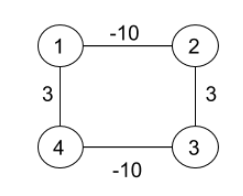
\includegraphics[width=0.3\textwidth]{synchronous-hopfield.png}
	\caption{Starting with 1 and 2 actives, in the next step 3 and 4 will be active. This network is not stable.}
\end{figure}

Trick for analysis: make a larger asynchronous network based on the network we want to analyse. Duplicate the units in two columns and only use non-zero weights between them.

\begin{figure}[H]
	\centering
	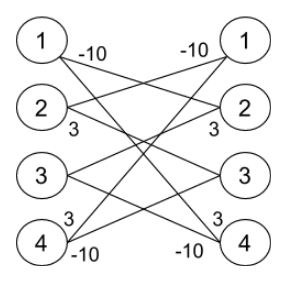
\includegraphics[width=0.3\textwidth]{hopfield-asynchronous-trick.png}
	\caption{Starting with 1 and 2 actives, we will end up with 3 and 4 active in the second column. First column represents $t=0$, second $t=1$. With synchronous updates, a Hopfield Network converges to a cycle of length 2 or to a stable state.}
\end{figure}

\begin{itemize}[noitemsep,nolistsep]
	\item Nodes can be updated synchronously or asynchronously.
	\item State: Set of units that are active, it can be seen as the activity vector.
	\item Dynamics: Units update their activity level.
	\item When a node is updated, weights are considered from all other active nodes, like with a perceptron.
	\item Asynchronous updates (greedy algorithm) converge to a stable state (sequential), but the converged state can depend on update order.
	\item Asynchronous is either in max-clique state if activity is in $\{0,1\}$ or min-cut if activities are in $\{-1,1\}$.
	\item Synchronous, parallel updates either also go to a stable state, just like asynchronous, or can get stuck in a pair of patterns (flipping or cyclic).
\end{itemize}


\end{document}
